\section{Calibration}
\label{sec:calibration}

%The first stage of the amplification chain is HEMT, whose added noise 
%dominates the noise from the readout electronics and could be 
%expressed in terms of an effective temperature \ta\ 
%(see Section~\ref{sec:intronoise}).
The noise is one of the most important 
parameters for the axion searches. Therefore, calibration for the HEMT is a 
crucial part in the operation of TASEH. In order to perform a calibration, 
the HEMT was connected to a heat source (resistors) instead of the cavity; 
various values of input currents were sent to the source to change its 
temperature monitored by a thermometer. The power from the source 
was delivered following the same transmission line as that in the axion 
data running
%: first to the HEMT, then to the amplifiers outside the DR at room 
%temperature, and finally to the signal analyzer.
The output power was fitted to a first-order polynomial, as a function of the source temperature, 
to extract the gain and added noise for the amplification chain. More details of the 
procedure can be found in Ref.~\cite{TASEHInstrumentation}. 

The calibration was carried out before, 
during, and after the data taking, which showed that the performance of the system
was stable over time. The average of the added noise \ta\ over 19 measurements 
has the lowest value of 1.9~K at the frequency of 4.8~GHz and the highest value of 
2.2~K at 4.72~GHz, as presented in Fig.~\ref{fig:hemtcalvsf}. 
The error bars are the RMS of \ta\ and the largest RMS was used to calculate 
the systematic uncertainty for the limits on \gagg. The light blue points in 
Fig.~\ref{fig:hemtcalvsf} are the noise from the axion data estimated by 
removing gain and subtracting the contribution from the cavity noise, assuming 
that the presence of a narrow signal in the data would have no effect on the 
estimation. A good agreement between the results from the calibration  
and the ones estimated from the axion data is shown. The biggest 
difference is 0.076~K in the frequency range during which the data were 
recorded after an earthquake. The source of the difference is not understood, 
therefore, the difference is quoted as a systematic uncertainty together 
with the RMS of the noise.

\begin{figure} [htbp]
  \centering
  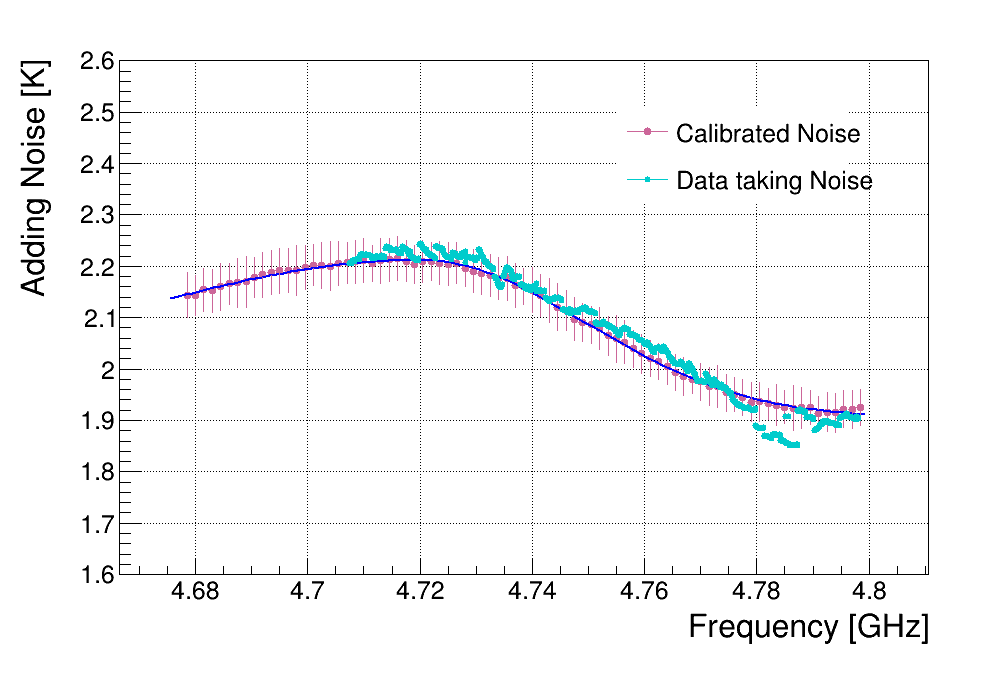
\includegraphics[width=0.4\textwidth,height = 0.25\textwidth]{figures/Avg_Noise_vs_Freq_run1to19_211118.png}
  \caption{The average added noise from the HEMT calibration (pink points) and 
 the noise estimated from the axion data (light blue points) as a function of frequency.}
  \label{fig:hemtcalvsf}
\end{figure}


  

